\chapterheading{6}{KIỂM THỬ VÀ ĐÁNH GIÁ}
\setcounter{section}{6}
\setcounter{subsection}{0}
\setcounter{subsubsection}{0}

\subsection{Mục tiêu và phạm vi đánh giá}
Chương này đánh giá tính đúng đắn của phép tổng hợp thời gian và phân tích ý nghĩa của các chỉ số dùng trong báo cáo. Phần thực nghiệm đã thực hiện là chạy bộ tính tham chiếu trên đầu vào tổng hợp, đối chiếu đáp án và kiểm tra các bất biến. Phần nhận biết từ video được trình bày như một quy trình đánh giá tiếp theo vì bộ dữ liệu hiện có chưa chứa video, nhãn tham chiếu độc lập hoặc dự đoán của mô hình.

Hai loại bằng chứng được sử dụng có mục đích khác nhau. Kết quả thực thi bộ tính cho biết chương trình có xử lý đúng các khoảng đầu vào đã xét hay không. Các số đếm và thời lượng có nhiễu cho phép kiểm tra công thức chỉ số và độ nhạy theo giả định. Không sử dụng mức nhiễu S1, S2, S3 như tên phương pháp hoặc như ba lần chạy thuật toán thị giác.

\begin{table}[H]
\centering\small
\caption{Nguồn dữ liệu và phạm vi kết luận của phần đánh giá}
\label{tab:evaluation-scope}
\begin{tabularx}{\textwidth}{p{3.1cm}p{3.1cm}X}
\toprule
Nhóm dữ liệu & Quy mô & Nội dung được kiểm chứng\\
\midrule
Kịch bản khoảng xác định & 24 trường hợp & Đáp án thời lượng và từ chối cấu hình sai\\
Khoảng ngẫu nhiên & 2.000 trường hợp & Đối chiếu hai cách tính và kiểm tra bất biến\\
Số đếm tổng hợp & Các khối độc lập & Precision, Recall, F1 và WPAR từ số đếm\\
Thời lượng có nhiễu & 12 phiên, 30 ca & MAE, MAPE và độ phân tán theo giả định\\
Video CCTV & Chưa có kết quả chạy & Chưa kết luận về nhận biết, theo dõi hoặc FPS\\
\bottomrule
\end{tabularx}
\end{table}

Các nhóm trên không được cộng thành một cỡ mẫu chung. Một ca tổng hợp có ba mức nhiễu vẫn là cùng một đầu vào tham chiếu. Tương tự, các phép biến đổi của một kịch bản kiểm thử dùng để kiểm tra tính ổn định của chương trình, không tạo thêm quan sát thực địa độc lập.

% Generated by generate_interval_evaluation.py; deterministic fixtures, not CCTV measurements.
\subsection{Kiểm tra tổng hợp khoảng thời gian bằng kịch bản xác định}
\label{sec:interval-evaluation}
Bộ dữ liệu bổ sung gồm 14 kịch bản có mốc bắt đầu, kết thúc và đáp án được xác định trước. Mục tiêu là kiểm tra phép hợp, giao, hiệu các tập khoảng và quy tắc hạn mức, bổ sung cho các số đếm và tổng thời lượng ở mục trước. Chương trình thực thi một bộ tính tham chiếu độc lập, chưa gọi bộ phát hiện, bộ theo dõi hoặc máy trạng thái của hệ thống triển khai. Vì vậy, kết quả đúng trên các kịch bản này chỉ xác nhận phép tính tham chiếu trong phạm vi đã xét.

Các khoảng được biểu diễn nửa kín $[s,e)$, đơn vị giây kể từ đầu ngày giả định. Mốc lớn hơn 86.400 biểu diễn ngày tiếp theo. Khoảng có độ dài bằng không được bỏ qua, khoảng có mốc kết thúc nhỏ hơn mốc bắt đầu bị từ chối. Các khoảng trùng và chồng lấn được hợp nhất trước khi tính thời lượng. Lịch làm việc hợp lệ được loại phần không quan sát được trước khi lấy giao với hiện diện và điện thoại.

\begin{table}[H]
\centering\small
\caption{Kết quả tính trên các kịch bản khoảng thời gian tổng hợp, đơn vị giây}
\label{tab:interval-checks}
\begin{tabularx}{\textwidth}{lXrrrr}
\toprule
Mã & Kịch bản & $T_{presence}$ & $T_{phone}$ & $T_{excess}$ & $T_{effective}$\\
\midrule
I01 & Không sử dụng điện thoại & 3600 & 0 & 0 & 3600\\
I02 & Dưới hạn mức & 3600 & 840 & 0 & 3600\\
I03 & Đúng hạn mức & 3600 & 900 & 0 & 3600\\
I04 & Vượt hạn mức 1 giây & 3600 & 901 & 1 & 3599\\
I05 & Khoảng chồng lấn và lặp & 3600 & 1100 & 200 & 3400\\
I06 & Điện thoại ngoài hiện diện & 1800 & 400 & 0 & 1800\\
I07 & Ca có khoảng nghỉ & 3600 & 600 & 0 & 3600\\
I08 & Loại khoảng mất quan sát & 3000 & 600 & 0 & 3000\\
I09 & Mất quan sát chồng lấn & 3200 & 0 & 0 & 3200\\
I10 & Ca qua nửa đêm & 3600 & 1200 & 300 & 3300\\
I11 & Tắt điều chỉnh thời gian & 3600 & 1200 & 300 & 3600\\
I12 & Không có lịch làm việc & 0 & 0 & 0 & 0\\
I13 & Khoảng độ dài bằng không & 200 & 0 & 0 & 200\\
I14 & Từ chối thời lượng âm & -- & -- & -- & --\\
\bottomrule
\end{tabularx}
\end{table}

Mười ba kịch bản hợp lệ khớp toàn bộ các đại lượng với đáp án đã xác định trước, còn I14 bị từ chối đúng quy tắc. Đây là mức bao phủ kịch bản, không phải tỉ lệ chính xác của mô hình thị giác. I05 cho thấy bản ghi lặp không làm tăng thời lượng. I07 loại phần điện thoại nằm trong giờ nghỉ. I08 và I09 loại lần lượt 600 và 400 giây mất quan sát, cho độ bao phủ tương ứng 83,33\% và 88,89\%. I11 vẫn ghi nhận phần vượt hạn mức nhưng không trừ khi chính sách điều chỉnh bị tắt. I12 có độ bao phủ không xác định vì tổng lịch bằng không, không tự gán bằng 100\%.

\subsection{Phân tích tác động của hạn mức trên cùng dòng thời gian}
Dòng thời gian minh họa tại Hình~\ref{fig:timeline-ui} có hai khoảng hiện diện: 08:05--12:00 và 13:05--17:15, tổng 485 phút. Bốn phiên điện thoại dài 8, 12, 20 và 5 phút, tổng 45 phút. Với hạn mức 15 phút, phần vượt là 30 phút và thời gian hiệu lực là 455 phút. Trên hình, phần vượt được tô theo thứ tự thời gian để giải thích phép trừ. Đây là quy ước hiển thị, không phải nhãn về năng suất từng đoạn.

\begin{table}[H]
\centering
\caption{Ảnh hưởng của hạn mức trên cùng dữ liệu tổng hợp, đơn vị phút}
\label{tab:allowance-sensitivity}
\begin{tabular}{rrrr}
\toprule
Hạn mức & Điện thoại & Phần vượt & Thời gian hiệu lực\\
\midrule
0 & 45 & 45 & 440\\
5 & 45 & 40 & 445\\
15 & 45 & 30 & 455\\
30 & 45 & 15 & 470\\
45 & 45 & 0 & 485\\
\bottomrule
\end{tabular}
\end{table}

Khi hạn mức tăng từ 0 đến tổng thời gian điện thoại, thời gian hiệu lực tăng cùng lượng, sau đó giữ ở mức hiện diện. Thay đổi này xuất phát hoàn toàn từ chính sách, không thể diễn giải thành cải thiện độ chính xác mô hình. Phân tích giúp phân biệt sai số quan sát với tác động của quy định áp dụng sau quan sát.

Tệp \texttt{data/interval\_evaluation/evaluation.json} công bố toàn bộ khoảng đầu vào, đáp án, kết quả và dữ liệu của hình minh họa. Có thể tái tạo bằng \texttt{python generate\_interval\_evaluation.py}. Bản kê đi kèm lưu mã SHA-256 của chương trình và dữ liệu. Các kịch bản không bao phủ chất lượng liên kết danh tính, điều kiện chuyển trạng thái, độ trễ hay tính đúng đắn của dịch vụ triển khai.


% Generated by evaluate_interval_arithmetic.py after assertions pass.
\subsection{Thực nghiệm tính toán với bộ đối chiếu độc lập}
\label{sec:computational-experiment}
Để mở rộng phạm vi kiểm thử ngoài các đáp án cố định, chương trình thực thi bộ tổng hợp trên 2.000 trường hợp ngẫu nhiên có hạt giống 20260919. Tám nhóm có quy mô bằng nhau, mỗi nhóm 250 trường hợp. Lịch danh định dài 4, 6 hoặc 8 giờ và có khoảng nghỉ 10 phút ở giữa. Các đầu mút được sinh trên lưới một giây, có thể nằm ngoài lịch 300 giây để kiểm tra thao tác cắt khoảng. Các khoảng ngẫu nhiên phục vụ phát hiện lỗi số học, không được dùng như phân phối hành vi nhân viên.

Bộ tính cần kiểm tra dùng phép sắp xếp, hợp nhất, giao và hiệu các khoảng. Bộ đối chiếu được cài đặt riêng, biểu diễn mỗi giây $[t,t+1)$ bằng một bit, dùng phép toán bit và đếm số bit còn lại. Bộ đối chiếu không gọi các hàm hợp nhất hoặc giao của mô-đun cần kiểm tra. Hai cách biểu diễn phải cho cùng sáu đại lượng: thời lượng lịch, hiện diện, điện thoại, mất quan sát, phần vượt và thời gian hiệu lực. Độ bao phủ được đối chiếu riêng. Cách đếm ô giây là chính xác đối với các đầu mút nguyên của tập này, không phải phép xấp xỉ cho mốc thời gian tùy ý.

\begin{table}[H]
\centering\small
\caption{Kết quả đối chiếu bộ tính khoảng với biểu diễn bit độc lập}
\label{tab:computational-checks}
\begin{tabularx}{\textwidth}{Xrr}
\toprule
Nhóm đầu vào & Số trường hợp & Khớp đáp án\\
\midrule
Khoảng phân bố ngẫu nhiên & 250 & 250\\
Lịch và hiện diện trùng & 250 & 250\\
Điện thoại chồng lấn & 250 & 250\\
Gián đoạn trong và ngoài ca & 250 & 250\\
Không có lịch & 250 & 250\\
Mất quan sát toàn ca & 250 & 250\\
Hạn mức bằng không & 250 & 250\\
Tắt điều chỉnh & 250 & 250\\
\midrule
Tổng & 2.000 & 2.000\\
\bottomrule
\end{tabularx}
\end{table}

Trong 2.000 trường hợp đã chạy, sai lệch giữa hai cách tính bằng không ở tất cả các đại lượng đối chiếu. Mỗi đầu vào còn được đảo thứ tự, nhân đôi bản ghi, dịch toàn bộ mốc thêm một ngày và chia mỗi khoảng thành hai đoạn liền kề. Cả bốn phép biến đổi đều giữ nguyên thời lượng và độ bao phủ, tương ứng 8.000 lượt kiểm tra. Việc tăng hạn mức thêm 300 giây cũng không làm giảm thời gian hiệu lực trong 2.000 lượt kiểm tra bổ sung. Các lượt biến đổi dùng lại đầu vào gốc, không được tính như những mẫu thực địa độc lập.

Sáu đầu vào phụ kiểm tra giá trị không hữu hạn, sai kiểu và sai số lượng đầu mút đều bị từ chối. Một trường hợp dùng mốc 0,25 và 1,75 giây cho thời lượng hiện diện 1,5 giây, điện thoại 1 giây, hạn mức 0,75 giây và hiệu lực 1,25 giây, khớp đáp án trực tiếp. Trường hợp này chỉ kiểm tra xử lý mốc lẻ, không mở rộng kết luận của bộ đối chiếu lưới một giây sang mọi số thực.

Kết quả cho thấy bộ tính tham chiếu bảo toàn các bất biến đã kiểm tra, đặc biệt là tính không phụ thuộc thứ tự và tính không cộng trùng. Kết quả không chứng minh máy trạng thái tạo đúng đầu vào, cũng không đánh giá độ chính xác của YOLOv8, ByteTrack hoặc FaceNet. Mã chạy, cấu hình sinh, từng đầu vào và kết quả được lưu trong \path{computational_evaluation/}. Tệp bản kê ghi phiên bản Python, hệ điều hành và mã SHA-256 của các tệp dùng trong lần chạy.


% Generated from data/synthetic_evaluation/evaluation.json. Do not edit numbers manually.
\subsection{Phân tích chỉ số trên bộ số liệu tổng hợp}
\subsubsection{Nguồn gốc và cấu trúc dữ liệu}
\label{sec:synthetic-origin}
Bộ dữ liệu trong phần này được tạo bằng chương trình với hạt giống ngẫu nhiên cố định 20260917. Dữ liệu gồm số đếm phân loại và các bản ghi thời lượng, không phải video đã chạy qua mô hình thị giác máy tính. Các tham số được chọn để bao phủ ca làm có độ dài khác nhau, trường hợp dưới và trên hạn mức điện thoại, khoảng mất quan sát và một số sai số lớn. Đây là các giả định thiết kế chưa được hiệu chỉnh theo dữ liệu thực địa.

Các bảng dưới đây được tính lại từ cùng tệp dữ liệu nguồn. Mã SYN-P và SYN-C nhận diện bản ghi tổng hợp. Các giá trị hiển thị được làm tròn đến số chữ số đã công bố, với trường hợp đúng nửa đơn vị làm tròn lên về độ lớn. Chỉ số tổng hợp được tính từ dữ liệu chưa làm tròn.

Năm khối dữ liệu độc lập gồm số đếm phát hiện người, số đếm hiện diện, số đếm sử dụng điện thoại, 12 phiên điện thoại và 30 ca. Không ghép các khối này thành một tập quan sát chung hoặc suy ra quan hệ nhân quả giữa chúng. Ba mức S1, S2 và S3 biểu diễn mức nhiễu tăng dần, không đại diện ba thuật toán đã được chạy.

\begin{table}[H]
\centering
\caption{Các giả định của bộ dữ liệu tổng hợp}
\label{tab:synthetic-assumptions}
\begin{tabularx}{\textwidth}{p{4.4cm}X}
\toprule
Thành phần & Quy tắc tạo dữ liệu\\
\midrule
Thời lượng ca & 4, 6 hoặc 8 giờ\\
Mất quan sát & 0, 30, 90 hoặc 180 giây, lưu riêng với vắng mặt\\
Hiện diện tham chiếu & 76--96\% thời gian có quan sát\\
Điện thoại trong ca & 0--2700 giây, có mẫu tại ngưỡng hạn mức\\
Hạn mức điện thoại & 900 giây mỗi ca, dùng để kiểm tra công thức\\
Nhiễu thời lượng hiện diện & Phân phối chuẩn với trung bình $-35$ giây, độ lệch chuẩn 65 giây\\
Nhiễu thời lượng điện thoại & Phân phối chuẩn với trung bình $-5$ giây, độ lệch chuẩn 25 giây\\
Trường hợp sai số lớn & Ca 10, 20 và 30 thêm sai lệch có độ lớn 180--330 giây\\
Mức nhiễu S1/S2/S3 & Nhân cùng sai lệch cơ sở lần lượt với 1, 2 và 4\\
\bottomrule
\end{tabularx}
\end{table}

Thời lượng được làm tròn đến giây và giới hạn trong miền hợp lệ. Thời gian điện thoại không vượt thời gian hiện diện, thời gian hiện diện không vượt thời gian có quan sát. Các ràng buộc này bảo đảm tính nhất quán số học, nhưng không xác nhận rằng phân phối nhiễu phản ánh một camera hoặc một mô hình cụ thể.

\subsubsection{Kiểm tra chỉ số phát hiện người bằng số đếm tổng hợp}
Đơn vị tham chiếu là một đối tượng người tại một thời điểm quan sát, không phải một khung hình. Bảng sử dụng 10.000 đối tượng tham chiếu. TP, FP và FN là số đếm được khai báo trong bộ tổng hợp để kiểm tra công thức Precision, Recall và F1. Tổng hợp được tính từ tổng số đếm, không lấy trung bình các tỉ lệ theo số khung hình.
\begin{table}[H]
\centering
\small
\caption{Chỉ số phát hiện người từ số đếm tổng hợp}
\label{tab:syn-person}
\begin{tabular}{lrrrrrr}
\toprule
Điều kiện & TP & FP & FN & P & R & F1\\
\midrule
Ít che khuất & 3063 & 91 & 137 & 0,971 & 0,957 & 0,964\\
Che khuất nhẹ & 2539 & 139 & 261 & 0,948 & 0,907 & 0,927\\
Che khuất vừa & 1987 & 184 & 413 & 0,915 & 0,828 & 0,869\\
Sát biên vùng & 1271 & 152 & 329 & 0,893 & 0,794 & 0,841\\
Tổng & 8860 & 566 & 1140 & 0,940 & 0,886 & 0,912\\
\bottomrule
\end{tabular}
\end{table}
Tên điều kiện và số đếm được khai báo để minh họa cách phân nhóm. Chỉ số ở hàng tổng được tính theo tổng TP, FP, FN, nhờ đó tránh sai lệch do lấy trung bình không trọng số giữa các nhóm có quy mô khác nhau.

\subsubsection{Kiểm tra chỉ số hiện diện trên cùng tập tham chiếu}
Mỗi kịch bản có 36.000 mẫu người--giây, trong đó 27.000 mẫu hiện diện và 9.000 mẫu vắng mặt. Khoảng mất quan sát không nằm trong tập phân loại này. Vì mỗi mẫu có độ dài một giây, FN chính là số giây vắng mặt giả và FP chính là số giây hiện diện giả.
\begin{table}[H]
\centering
\small
\caption{Chỉ số hiện diện trên ba kịch bản nhiễu tổng hợp}
\label{tab:syn-presence}
\begin{tabular}{lrrrrrrr}
\toprule
Mức & TP & FP (s) & FN (s) & TN & P & R & F1\\
\midrule
S1 & 26190 & 430 & 810 & 8570 & 0,984 & 0,970 & 0,977\\
S2 & 25110 & 810 & 1890 & 8190 & 0,969 & 0,930 & 0,949\\
S3 & 23490 & 1440 & 3510 & 7560 & 0,942 & 0,870 & 0,905\\
\bottomrule
\end{tabular}
\end{table}
\begin{figure}[H]
\centering
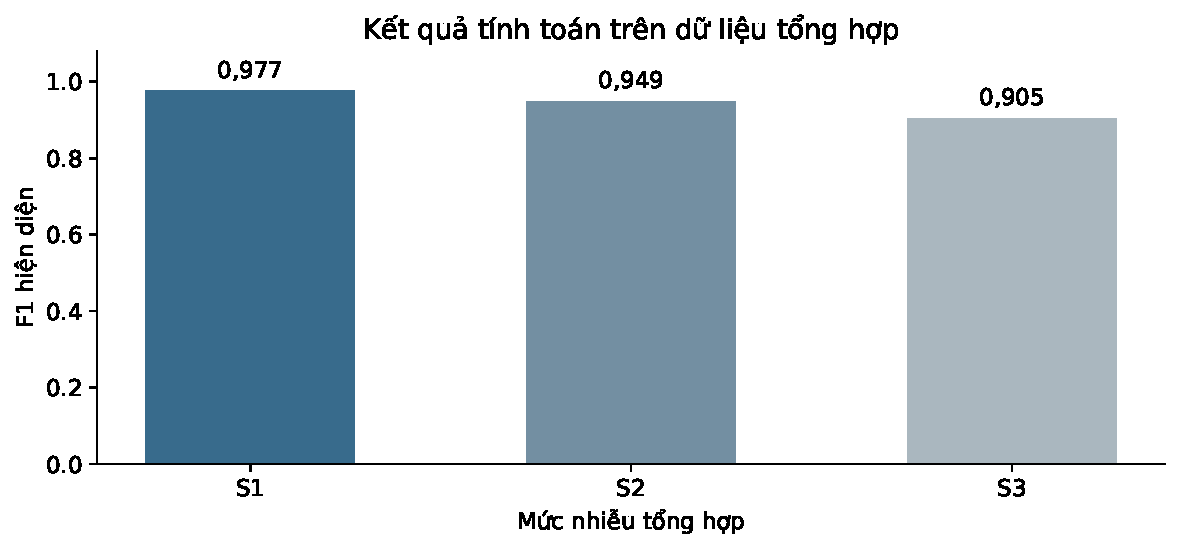
\includegraphics[width=0.88\textwidth]{Images/synthetic_presence_f1.pdf}
\caption{F1 hiện diện tính từ số đếm tổng hợp}
\label{fig:synthetic-presence}
\end{figure}
Ba hàng có cùng số mẫu dương và âm, nên thay đổi Recall có thể đối chiếu trực tiếp với số giây vắng mặt giả. F1 giảm khi tăng các số đếm lỗi theo giả định. S1, S2 và S3 không tương ứng với các cấu hình thuật toán trong quy trình đánh giá video.

\subsubsection{Kiểm tra chỉ số sử dụng và liên kết điện thoại}
Mỗi điều kiện có 3.000 mẫu người--giây. Bốn điều kiện đầu có 1.000 mẫu sử dụng và 2.000 mẫu không sử dụng. Điều kiện chỉ đặt điện thoại trên bàn có toàn bộ 3.000 mẫu âm, do đó Recall và F1 không được báo cáo. Tỉ lệ dương tính giả được tính theo $FPR=FP/(FP+TN)$.
\begin{table}[H]
\centering
\small
\caption{Phân loại sử dụng điện thoại từ số đếm tổng hợp}
\label{tab:syn-phone}
\begin{tabular}{lrrrrrrr}
\toprule
Điều kiện & TP & FP & FN & P & R & F1 & FPR\\
\midrule
Một người & 920 & 73 & 80 & 0,926 & 0,920 & 0,923 & 0,037\\
Nhiều người & 845 & 110 & 155 & 0,885 & 0,845 & 0,864 & 0,055\\
Che khuất tay & 728 & 132 & 272 & 0,847 & 0,728 & 0,783 & 0,066\\
Gần hai người & 760 & 148 & 240 & 0,837 & 0,760 & 0,797 & 0,074\\
Chỉ đặt trên bàn & 0 & 64 & 0 & 0,000 & -- & -- & 0,021\\
\bottomrule
\end{tabular}
\end{table}
WPAR sử dụng đơn vị sự kiện đã được gán người, khác với đơn vị người--giây của bảng phân loại. Các số đếm sự kiện bên dưới là một khối giả định riêng, không được dùng thay mẫu số của Precision hoặc Recall. Trường hợp không có sự kiện được gán có WPAR không xác định, ký hiệu bằng dấu gạch ngang.
\begin{table}[H]
\centering
\small
\caption{Sai gán người trên các sự kiện điện thoại tổng hợp}
\label{tab:syn-owner}
\begin{tabular}{lrrr}
\toprule
Điều kiện & Đã gán & Gán sai & WPAR\\
\midrule
Một người & 80 & 1 & 0,013\\
Nhiều người & 110 & 4 & 0,036\\
Che khuất tay & 95 & 6 & 0,063\\
Gần hai người & 105 & 9 & 0,086\\
Chỉ đặt trên bàn & 0 & 0 & --\\
\bottomrule
\end{tabular}
\end{table}
\subsubsection{Sai số thời lượng của 12 phiên điện thoại tổng hợp}
Thời lượng tham chiếu của 12 phiên được khai báo trong dữ liệu nguồn. Sai lệch được lấy từ phân phối chuẩn có trung bình $-2$ giây và độ lệch chuẩn $6+0{,}035T$ giây, với $T$ là thời lượng tham chiếu. Các giả định này tạo cả sai số tăng và giảm thời lượng, chưa mô tả sai số đo được của mô hình.
\begin{table}[H]
\centering
\small
\caption{Toàn bộ 12 phiên điện thoại tổng hợp, đơn vị giây}
\label{tab:syn-phone-duration}
\begin{tabular}{lrrr}
\toprule
Mã phiên & Tham chiếu & Ước lượng tổng hợp & Sai số có dấu\\
\midrule
SYN-P01 & 34 & 24 & -10\\
SYN-P02 & 49 & 39 & -10\\
SYN-P03 & 76 & 92 & +16\\
SYN-P04 & 123 & 118 & -5\\
SYN-P05 & 188 & 185 & -3\\
SYN-P06 & 247 & 256 & +9\\
SYN-P07 & 326 & 334 & +8\\
SYN-P08 & 418 & 432 & +14\\
SYN-P09 & 507 & 482 & -25\\
SYN-P10 & 633 & 681 & +48\\
SYN-P11 & 746 & 764 & +18\\
SYN-P12 & 858 & 846 & -12\\
\bottomrule
\end{tabular}
\end{table}
MAE tính trên toàn bộ 12 phiên là 14,83 giây/phiên, trung vị sai số tuyệt đối là 11,00 giây và sai số tuyệt đối lớn nhất là 48 giây. Các giá trị này có thể tính lại trực tiếp từ bảng, không suy ra từ một tập mẫu chưa công bố.

\subsubsection{Sai số thời gian hiệu lực trên 30 ca tổng hợp}
Mỗi ca có thời lượng hiện diện và điện thoại tham chiếu. Sau khi bổ sung nhiễu, chương trình tính lại phần vượt hạn mức và thời gian hiệu lực cho từng mức S1, S2, S3 bằng cùng công thức ở Chương 1. Sai số được tính trên thời gian hiệu lực của cùng một ca. Khoảng mất quan sát được báo riêng, không tự động cộng vào hiện diện hoặc diễn giải là vắng mặt.
\begin{table}[H]
\centering
\small
\caption{Sai số thời gian hiệu lực trên 30 ca tổng hợp}
\label{tab:syn-worktime}
\begin{tabular}{lrrrrr}
\toprule
Mức & MAE (s/ca) & MAPE (\%) & Trung vị (s) & P95 (s) & Max (s)\\
\midrule
S1 & 73,40 & 0,44 & 42,50 & 253,50 & 306\\
S2 & 146,93 & 0,87 & 85,00 & 507,10 & 612\\
S3 & 295,80 & 1,76 & 169,00 & 1028,60 & 1224\\
\bottomrule
\end{tabular}
\end{table}
P95 sử dụng nội suy tuyến tính tại vị trí $(N-1)\times0{,}95$ trong dãy sai số tuyệt đối đã sắp tăng dần. MAPE chỉ tính trên thời lượng tham chiếu dương. Trong bộ này, cả 30 ca đều đáp ứng điều kiện. Các mức nhiễu sử dụng chung sai lệch cơ sở, vì vậy không được xem là các lần thử độc lập để kiểm định ưu thế thuật toán.
\begin{figure}[H]
\centering
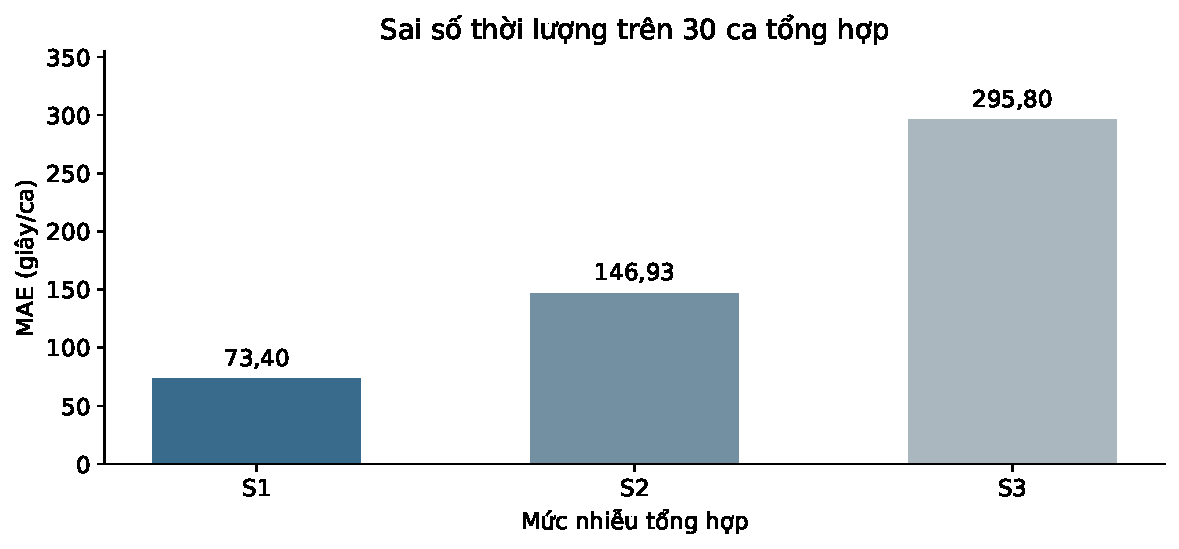
\includegraphics[width=0.88\textwidth]{Images/synthetic_time_mae.pdf}
\caption{MAE thời gian hiệu lực theo mức nhiễu tổng hợp}
\label{fig:synthetic-mae}
\end{figure}
\begin{figure}[H]
\centering
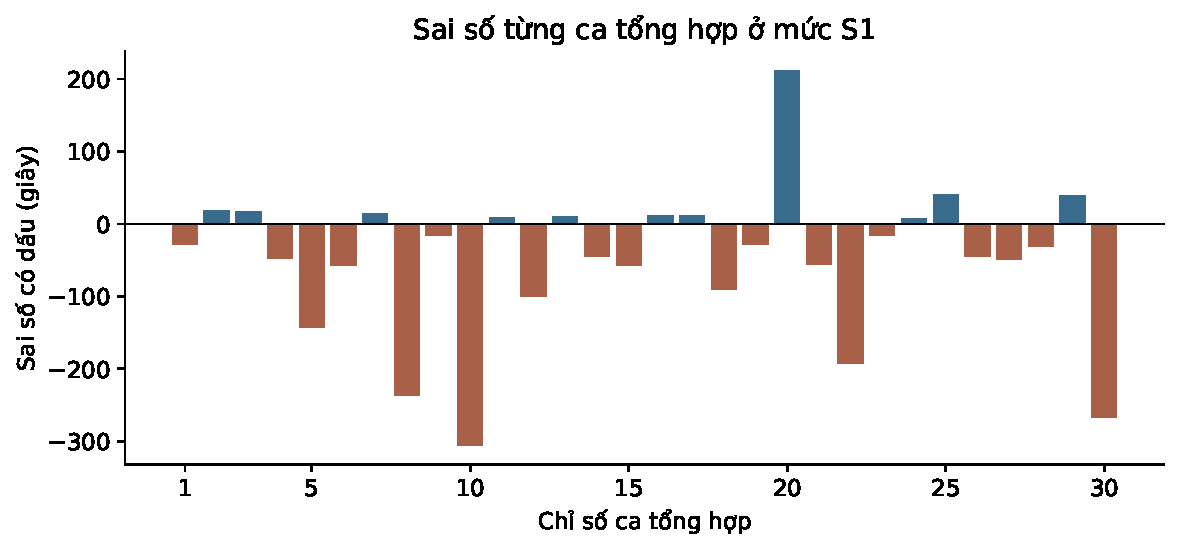
\includegraphics[width=0.88\textwidth]{Images/synthetic_shift_errors.pdf}
\caption{Sai số có dấu của 30 ca tổng hợp ở mức S1}
\label{fig:synthetic-errors}
\end{figure}
Phụ lục E công bố đủ 30 ca ở mức S1. Tệp dữ liệu nguồn lưu cả ba mức nhiễu cùng thời gian điện thoại trước và sau nhiễu. Mẫu không sử dụng điện thoại, mẫu đúng hạn mức và mẫu vừa vượt hạn mức giúp kiểm tra tính liên tục của phép điều chỉnh thời gian. Khối dữ liệu này chỉ chứa tổng thời lượng, không có mốc phiên để phân tích sai số biên. Kiểm thử phép xử lý khoảng được trình bày riêng tại mục~\ref{sec:interval-evaluation}.

\subsubsection{Lưu trữ và tái tạo số liệu}
Tệp \path{data/synthetic_evaluation/evaluation.json} lưu toàn bộ số đếm, thời lượng và chỉ số. Bản kê đi kèm công bố hạt giống, giả định, quy mô và mã SHA-256. Bộ dữ liệu giữ nguyên 12 phiên và 30 ca đã có, các giá trị không được thay đổi để tạo mức sai số thuận lợi hơn. Chạy \texttt{python generate\_synthetic\_evaluation.py} để tạo lại các bảng và hình.



\subsection{Thảo luận kết quả và giới hạn suy luận}
Thực nghiệm tính toán xác nhận bộ tổng hợp tham chiếu xử lý đúng các đáp án cố định và không phát sinh chênh lệch so với bộ đối chiếu độc lập trong tập đã chạy. Các tình huống trùng khoảng, mất quan sát và thay đổi hạn mức có ý nghĩa trực tiếp đối với đặc tả nghiệp vụ. Tuy nhiên, một phép tổng hợp đúng vẫn có thể tạo báo cáo sai nếu khoảng hiện diện hoặc người sử dụng điện thoại ở đầu vào đã bị nhận biết sai.

Kết quả MAE của bộ thời lượng tổng hợp phản ánh độ lớn nhiễu đã đưa vào. Chẳng hạn, mức S3 được tạo bằng cách nhân sai lệch cơ sở với hệ số lớn hơn S1, vì vậy sai số lớn hơn là hệ quả của thiết kế dữ liệu. Các giá trị này phù hợp để kiểm tra cách tính và biểu diễn chỉ số, nhưng không chứng minh thành phần theo dõi hoặc máy trạng thái làm giảm sai số. Tương tự, các nhóm che khuất trong bảng số đếm là tên tình huống giả định, chưa phải các phân tầng được gán nhãn từ video.

Giới hạn chính gồm phạm vi đầu vào tổng hợp, số kịch bản hữu hạn và việc chỉ thực thi bộ tính tham chiếu. Bộ đối chiếu lưới một giây kiểm tra chính xác các mốc nguyên đã sinh, nhưng không bao phủ mọi cấu hình thời gian có thể có. Các bước tạo khoảng từ khung hình, xác minh danh tính, xử lý sự kiện qua mạng và tích hợp cơ sở dữ liệu cần được kiểm thử riêng.

\subsection{Quy trình đánh giá trên video có nhãn tham chiếu}
\label{sec:video-evaluation-plan}
\subsubsection{Thu thập và phân chia dữ liệu}
Quy trình đề xuất sử dụng camera cố định quan sát nhiều vị trí làm việc. Mỗi phiên phải lưu mã video, thời lượng, độ phân giải, tốc độ khung hình, vị trí camera, sơ đồ ROI và điều kiện ánh sáng. Các kịch bản gồm người ngồi ổn định, nhiều người vào ra, giao nhau, che khuất, chuyển vùng, người khác ngồi vào bàn được gán, điện thoại trên bàn, điện thoại gần hai người và gián đoạn nguồn.

Dữ liệu được chia theo phiên quay, tránh đưa các khung hình gần nhau của cùng một phiên vào cả tập hiệu chỉnh và tập kiểm tra. Tỉ lệ 60/20/20 có thể dùng khi số phiên đủ lớn, nhưng thời lượng và số phiên thực tế của từng tập phải được công bố. Nếu chỉ dùng trọng số có sẵn, phần phát triển phục vụ khảo sát cấu hình. Tập kiểm tra chỉ được chạy sau khi khóa cấu hình và không được dùng để chọn ngưỡng.

\subsubsection{Quy tắc gán nhãn}
Nhãn cần gồm hộp bao và mã người cho tập khung hình đánh giá theo dõi, khoảng hiện diện, khoảng sử dụng điện thoại và người sử dụng tương ứng. Nhãn thời lượng có dạng $[s,e)$ trên trục thời gian của video. Điện thoại xuất hiện trong ảnh không đủ để gán nhãn đang sử dụng, cần dấu hiệu tương tác có thể quan sát. Trường hợp không đủ bằng chứng được ghi UNKNOWN, còn mất nguồn được ghi UNOBSERVED.

Một tập con có che khuất, giao nhau hoặc biên vào ra được hai người gán độc lập. Độ đồng thuận về nhãn loại có thể dùng hệ số kappa của Cohen \cite{cohen}, còn mốc thời gian được đối chiếu bằng sai lệch giây và IoU theo thời gian. Bất đồng được xem xét theo quy tắc đã thống nhất, lưu lý do điều chỉnh và không sửa nhãn chỉ để khớp dự đoán mô hình. Phụ lục C trình bày lược đồ nhãn đề xuất.

\subsubsection{So sánh phương pháp và loại bỏ thành phần}
Ba cấu hình chính gồm: YOLOv8 kết hợp ROI theo từng khung hình, YOLOv8 kết hợp ByteTrack và ROI, và chuỗi xử lý đầy đủ có xác minh danh tính cùng máy trạng thái. Các cấu hình phải dùng cùng video, bộ trọng số và quy tắc lấy mẫu để khác biệt có thể quy về thành phần được khảo sát.

Thí nghiệm loại bỏ thành phần khảo sát riêng FSM hiện diện, truy hồi mốc thời gian, xác minh danh tính và quy tắc liên kết điện thoại. Mỗi lần chỉ thay thành phần đang xét. Với hiện diện, chỉ số chính là MAE thời lượng và số giây hiện diện giả, vắng mặt giả. Với điện thoại, chỉ số chính là MAE thời lượng, WPAR và tỉ lệ sự kiện được gán người. Khi ngưỡng chặt hơn làm giảm gán nhầm nhưng tăng UNKNOWN, cả hai tác động đều phải được báo cáo.

\subsubsection{Tổng hợp và phân tích kết quả}
Chỉ số phát hiện phải kèm ngưỡng IoU, ngưỡng độ tin cậy và quy tắc ghép hộp một-một. Chỉ số thời lượng cần công bố số phiên hoặc số người--ca, MAE, trung vị, P95 và sai số lớn nhất. Kết quả được phân nhóm theo số người, mức che khuất, vùng ROI, kích thước điện thoại và điều kiện ánh sáng khi mỗi nhóm có đủ dữ liệu.

Vì các khung hình trong cùng phiên phụ thuộc nhau, việc ước lượng khoảng tin cậy bằng bootstrap nên lấy mẫu lại theo phiên hoặc theo cụm quan sát phù hợp \cite{efron}. Khi so sánh hai cấu hình trên cùng phiên, dùng chênh lệch sai số theo cặp. Quy mô mẫu và cách lấy mẫu phải được công bố, tránh suy luận ý nghĩa thống kê từ số lượng khung hình lớn nhưng chỉ thuộc một vài phiên.

\subsection{Kiểm thử tích hợp và hiệu năng đề xuất}
\subsubsection{Tính nhất quán của dữ liệu}
Phụ lục B liệt kê các ca kiểm thử dự kiến cho chuỗi tích hợp. Những trường hợp ưu tiên là sự kiện gửi lại, đảo thứ tự, mất xác nhận ACK, khởi động lại ứng dụng camera và mất kết nối bảng điều khiển. Kết quả cần được đối chiếu bằng mã sự kiện, khoảng thời gian và bản tổng hợp cuối cùng, thay vì chỉ dựa vào thông báo chương trình đã phục hồi.

\begin{table}[H]
\centering\small
\caption{Các kiểm thử tích hợp ưu tiên và bằng chứng cần thu}
\label{tab:e2e-tests}
\begin{tabularx}{\textwidth}{p{3.1cm}X X}
\toprule
Tình huống & Kết quả mong đợi & Bằng chứng\\
\midrule
Gửi lại cùng sự kiện & Không nhân đôi khoảng hoặc thời lượng & Mã sự kiện và bản tổng hợp\\
Mất mạng truyền dữ liệu & Giữ sự kiện cục bộ, đồng bộ khi nối lại & Hàng đợi, ACK và số thứ tự\\
Mất nguồn video & Ghi thời gian không quan sát được & Nhật ký nguồn và độ bao phủ\\
Khởi động lại ứng dụng & Phiên mới, không tái dùng mã quỹ đạo cũ & Mã phiên và các khoảng đã đóng\\
Truy cập khác tổ chức & Từ chối dữ liệu ngoài phạm vi quyền & Phản hồi API và nhật ký kiểm toán\\
Nhiều ca trong ngày & Áp dụng hạn mức riêng từng ca & Kết quả ca và tổng ngày\\
\bottomrule
\end{tabularx}
\end{table}

Đặc biệt, mất mạng từ thiết bị biên đến máy chủ không đồng nghĩa với mất khả năng quan sát. Nếu video vẫn được xử lý và sự kiện được lưu cục bộ, thời lượng có thể được khôi phục sau đồng bộ. Chỉ khoảng không có dữ liệu quan sát hợp lệ mới được đưa vào $T_{unobserved}$. Phân biệt này tránh giảm độ bao phủ chỉ vì bảng điều khiển tạm mất kết nối.

\subsubsection{Đo độ trễ và tài nguyên}
Đánh giá hiệu năng cần ghi thiết bị, hệ điều hành, phiên bản thư viện, trọng số, kích thước đầu vào và chính sách lấy mẫu. Sau giai đoạn khởi động, đo riêng giải mã, tiền xử lý, suy luận, theo dõi, xử lý trạng thái và truyền dữ liệu. FPS thu nhận và FPS xử lý phải được tách biệt. Độ trễ đầu-cuối được đo trên toàn đường đi của cùng khung hình hoặc sự kiện.

Đối với chuỗi tuần tự, trung bình của tổng thời gian bằng tổng trung bình các thành phần, nhưng P95 của tổng không bằng tổng P95 thành phần. Khi các công đoạn chạy song song, thông lượng còn phụ thuộc nút thắt và hàng đợi. Các đại lượng này không thể suy ra từ số đếm tổng hợp hoặc kết quả kiểm thử bộ tính thời gian, nên báo cáo hiện tại chưa gán số FPS hoặc độ trễ cho hệ thống CCTV.

\subsection{Tái lập kết quả}
Các lệnh dưới đây tạo lại hình, bảng, dữ liệu và báo cáo kiểm tra nguồn:
\begin{Verbatim}[fontsize=\small,breaklines=true]
python make_figures.py
python check_report_sources.py
\end{Verbatim}
Lệnh đầu chạy chương trình vẽ sơ đồ, sinh bộ số liệu tổng hợp, kiểm tra các kịch bản xác định và thực thi 2.000 trường hợp đối chiếu. Từng bộ dữ liệu có bản kê ghi giả định hoặc cấu hình cùng mã SHA-256. Các phép khẳng định trong chương trình phải hoàn tất trước khi tạo bảng kết quả. Lệnh thứ hai kiểm tra liên kết LaTeX, tài liệu tham khảo và sự khớp nhau giữa tệp với bản kê, không thay thế kiểm tra bố cục PDF.

\subsection{Kết luận chương}
Kết quả đã thực hiện gồm kiểm thử 24 kịch bản xác định, đối chiếu 2.000 đầu vào ngẫu nhiên và kiểm tra các bất biến của bộ tính thời gian. Hai mươi kịch bản hợp lệ khớp đáp án, bốn đầu vào sai bị từ chối và không ghi nhận chênh lệch với bộ đối chiếu độc lập. Các bảng số đếm, 12 phiên và 30 ca tổng hợp được tính lại từ nguồn để bảo đảm nhất quán số học. Bằng chứng hiện có hỗ trợ kết luận về bộ tính tham chiếu và cách tính chỉ số. Độ chính xác nhận biết, khả năng theo dõi và hiệu năng hệ thống tích hợp cần được xác định bằng quy trình video có nhãn đã trình bày.
